\begin{figure}[h!]
   \centering
   \begin{subfigure}[b]{0.4\textwidth}
      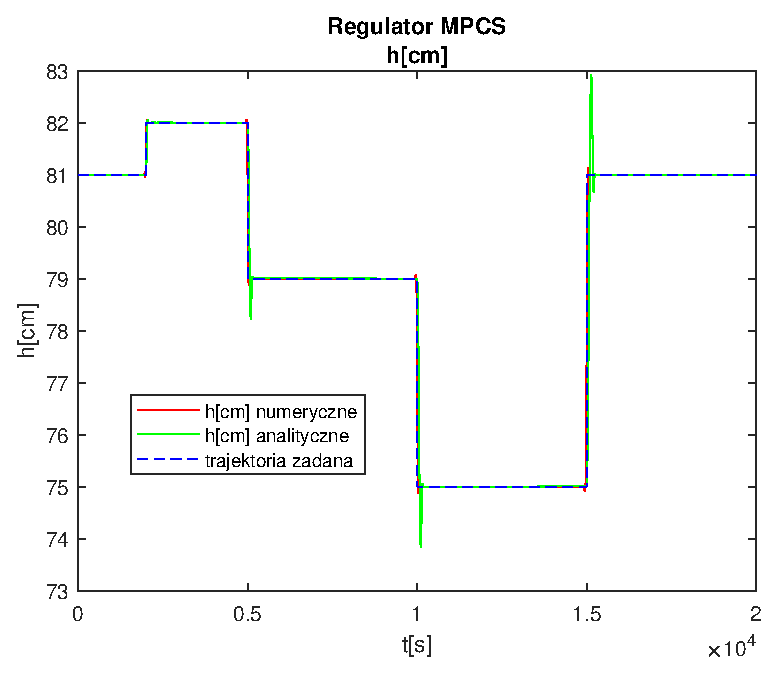
\includegraphics[width=1\linewidth]{img/MPCSnumRK/MPCSRKHN100Nu50l50.eps}
      \caption{}
      \label{fig:fig:MPCSRKN100Nu50l501}
   \end{subfigure}
       
   \begin{subfigure}[b]{0.4\textwidth}
      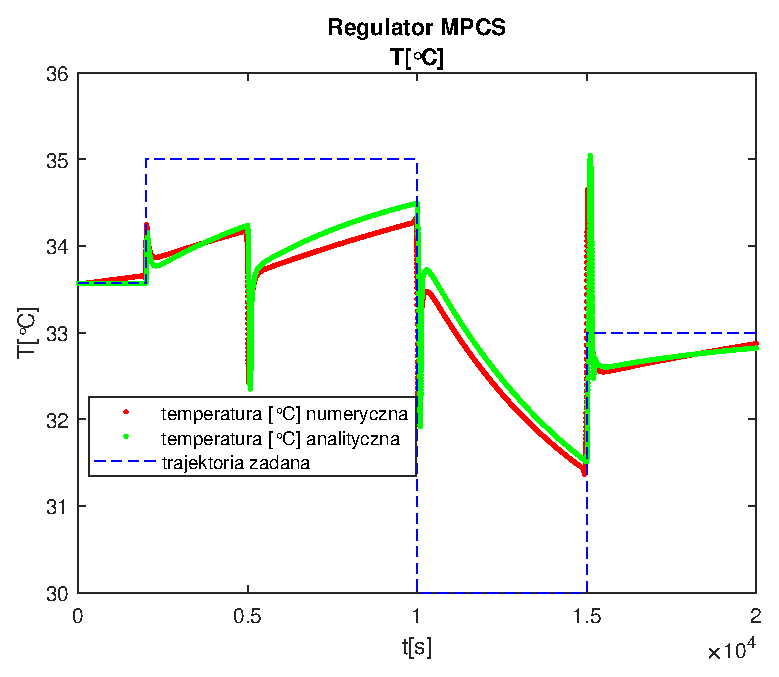
\includegraphics[width=1\linewidth]{img/MPCSnumRK/MPCSRKTN100Nu50l50.eps}
      \caption{}
      \label{fig:fig:MPCSRKN100Nu50l502}
   \end{subfigure}
       
   \begin{subfigure}[b]{0.4\textwidth}
      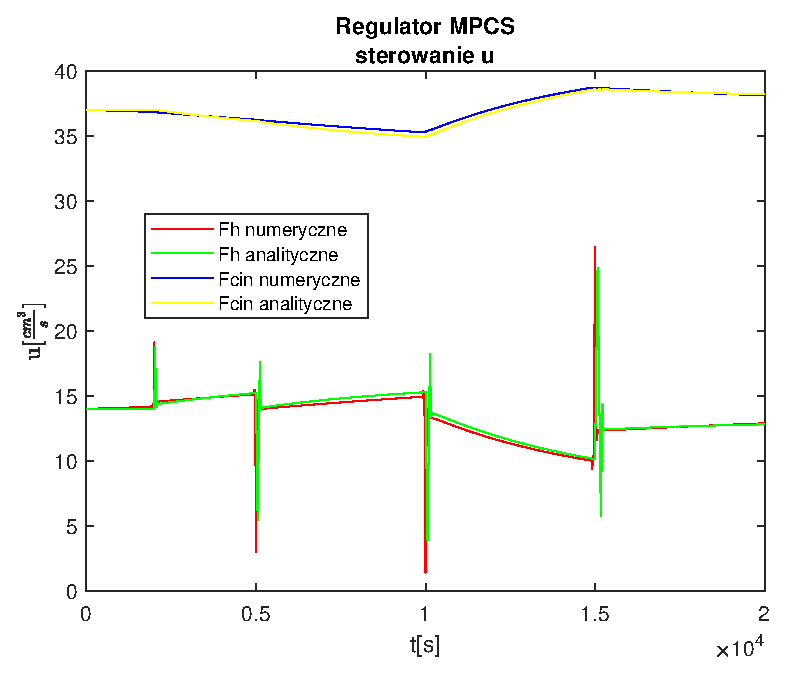
\includegraphics[width=1\linewidth]{img/MPCSnumRK/MPCSRKControlN100Nu50l50.eps}
      \caption{}
      \label{fig:fig:MPCSRKN100Nu50l503}
   \end{subfigure}
       
   \caption{Wykresy dla regulatora MPCS, obiekt nieliniowy, $N = 100$, $N_u = 50$, $\lambda = 0.5$.}
   \label{fig:MPCSRKN100Nu50l50}
\end{figure}
           
